\section{Connectivity to DHT11 sensor}
The DHT11 sensor is a temperature and humidity sensor and a 3-wire module: VCC (power), GND (ground) and DATA.\\
\begin{figure}[!ht]%
    \centering
    \subfloat[\centering Connectivity Diagram]{{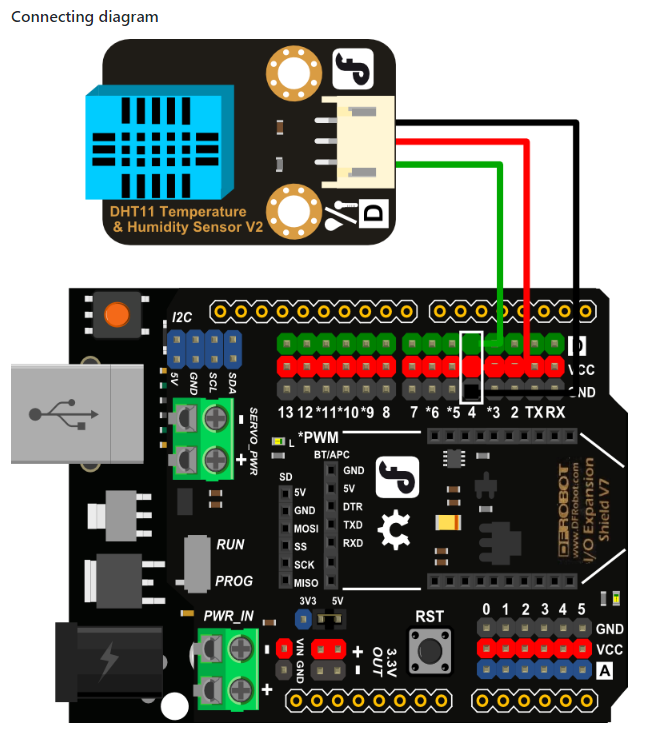
\includegraphics[scale=0.2]{images/connectingdiagram.png}}}%
    \qquad
    \subfloat[\centering Set up on NRF52840 board]{{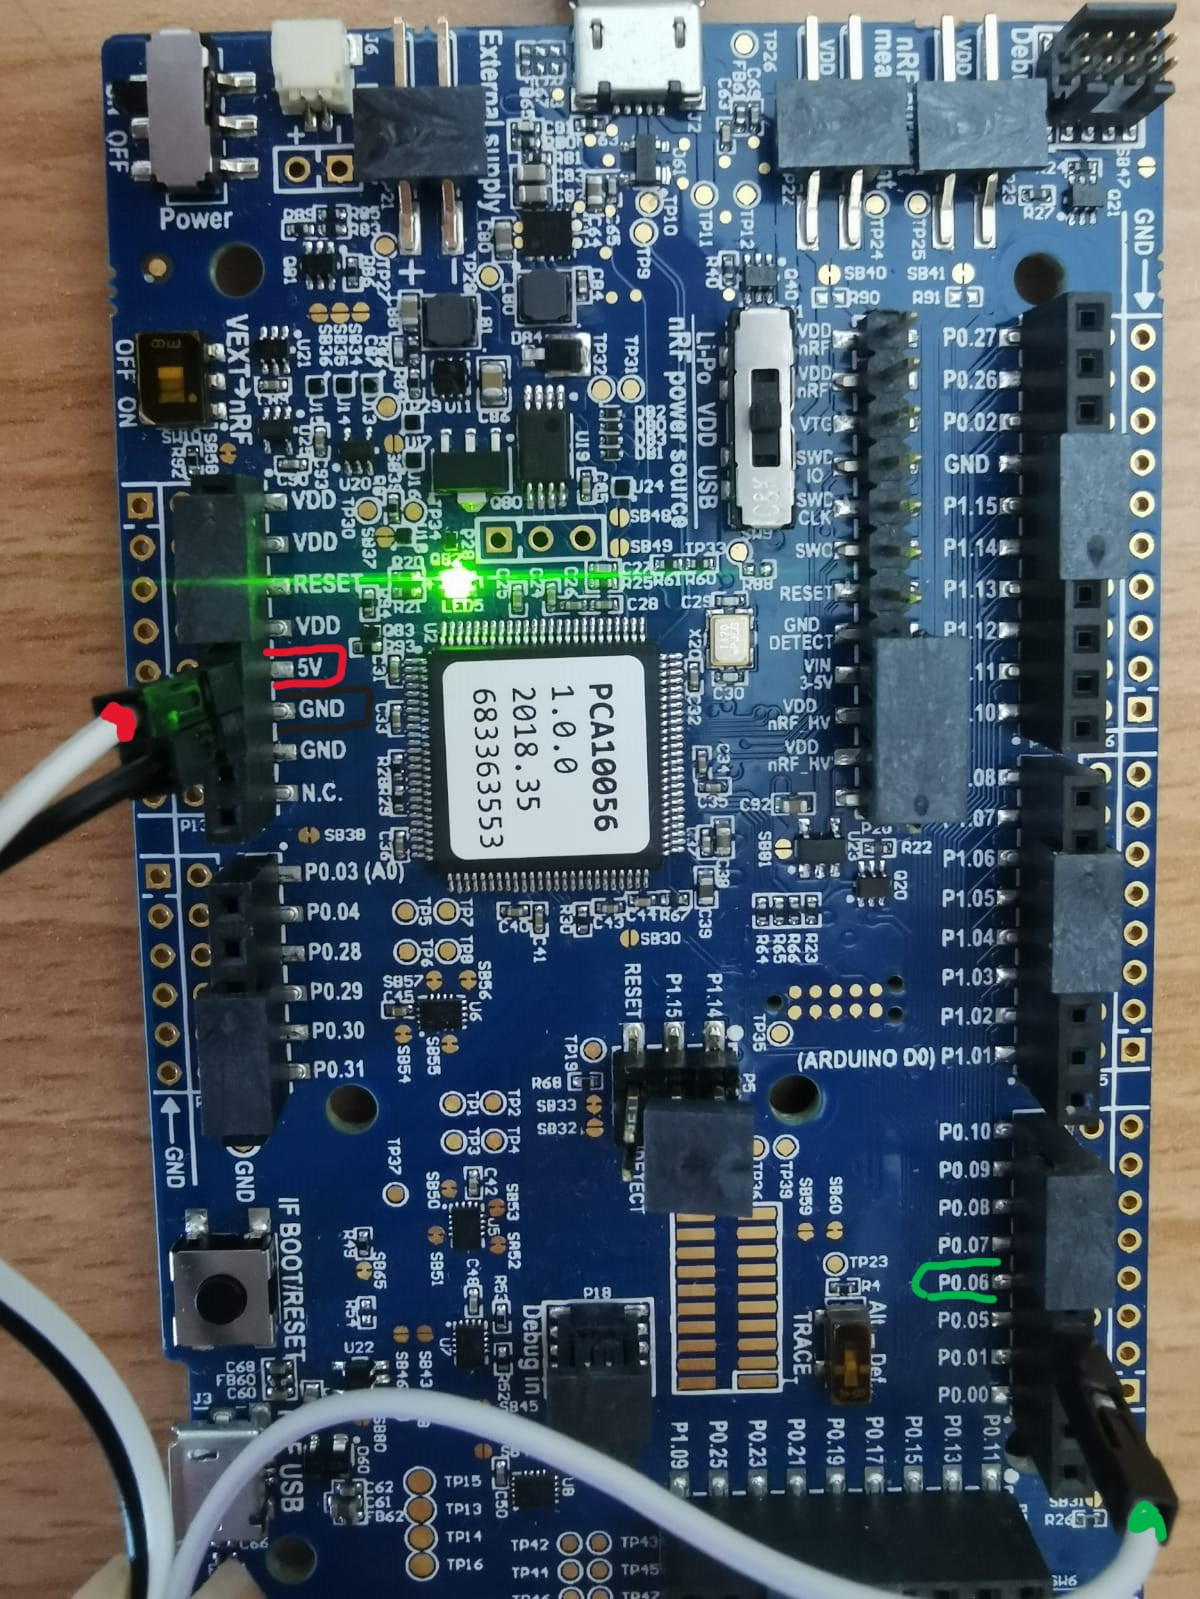
\includegraphics[scale=0.1]{images/ConnectivityToBoard.jpeg}}}%
    \caption{Connectivity of the DHT11 to the board}%
    \label{fig:example}%
\end{figure}
According to the specifications of the DHT11 sensor and considering that the board was connected by cable to the computer we knew that we could connect the VCC cable to either 3.5V or 5V. On our NRF52840 board however only the 5V was available. 
Regarding the data wire, we found that a possible option was to connect it to the GPIO14 (DTX). On the NRF52840 it corresponds to the P0.06. And the corresponding raw pin of the GPIO14 was 14. 
